% ============================================================================
% CSCE 763: Digital Image Processing - Homework 3 Solutions
% ============================================================================

\documentclass[12pt]{article}

% ============================================================================
% PACKAGE IMPORTS
% ============================================================================
\usepackage{amsmath}
\usepackage{amssymb}
\usepackage{graphicx}
\usepackage{tikz}
\usepackage[margin=1in]{geometry}
\usepackage{xcolor}
\usepackage{enumitem}
\usepackage{tcolorbox}
\usepackage{fancyhdr}
\usepackage{booktabs}
\usepackage{array}
\usepackage{colortbl}
\usepackage{float}

% ============================================================================
% HEADER AND FOOTER SETUP
% ============================================================================
\pagestyle{fancy}
\setlength{\headheight}{14.5pt}
\fancyhf{}

\fancyhead[L]{Page \thepage}
\fancyhead[C]{CSCE 763}
\fancyhead[R]{J.C. Vaught}

\renewcommand{\headrulewidth}{0pt}

% ============================================================================
% TIKZ LIBRARIES
% ============================================================================
\usetikzlibrary{shapes.geometric, arrows.meta, positioning, patterns, calc}

% --- USC Brand Colors ---
\definecolor{USC_Garnet}{HTML}{73000A}
\definecolor{USC_Sandstorm}{HTML}{FFF2E3}
\definecolor{USC_Black90}{HTML}{363636}
\definecolor{USC_Black70}{HTML}{5C5C5C}
\definecolor{USC_Black50}{HTML}{A2A2A2}
\definecolor{USC_Black10}{HTML}{ECECEC}
\definecolor{USC_Horseshoe}{HTML}{65780B}
\definecolor{USC_Atlantic}{HTML}{466A9F}
\definecolor{USC_Congaree}{HTML}{1F414D}
\definecolor{USC_Rose}{HTML}{CC2E40}
\definecolor{USC_Grass}{HTML}{CED318}

% Graphics path
\graphicspath{{figures/}}

% ============================================================================
% CUSTOM COLORED BOXES
% ============================================================================
\newtcolorbox{stepbox}[1][Step]{
  colback=white,
  colframe=USC_Garnet,
  fonttitle=\bfseries,
  title={#1},
  sharp corners,
  colbacktitle=USC_Garnet,
  coltitle=white,
}

\newtcolorbox{resultsbox}{
  colback=white,
  colframe=USC_Horseshoe,
  fonttitle=\bfseries,
  title=Results,
  sharp corners,
  colbacktitle=USC_Horseshoe,
  coltitle=white,
}

% ============================================================================
% CUSTOM QUESTION AND PART COMMANDS
% ============================================================================
\newcommand{\question}[1]{%
  \clearpage
  \vspace{0.5cm}
  {\noindent\normalsize \textbf{#1}}
  \vspace{0.2cm}
  \hrule
  \vspace{0.1cm}
  \hrule
  \vspace{0.3cm}
}

\newcommand{\questionpart}[1]{%
  \clearpage
  \vspace{0.5cm}
  {\noindent\normalsize \textbf{#1}}
  \vspace{0.2cm}
  \hrule
  \vspace{0.1cm}
  \hrule
  \vspace{0.3cm}
}

% ============================================================================
% DOCUMENT INFORMATION
% ============================================================================

\title{CSCE 763: Digital Image Processing \\ Homework \#3}
\author{Instructor: Spring 2026 \\ University of South Carolina \\ \textit{Solutions by: J.C. Vaught}}
\date{Due: 1:15 pm EST, Tuesday, Feb 17}

% ============================================================================
% BEGIN DOCUMENT
% ============================================================================

\begin{document}

\maketitle
\setlength{\parindent}{0pt}

\setlist[enumerate,1]{label=\arabic*.}
\setlist[enumerate,2]{label=(\alph*)}

% ============================================================================
% TABLE OF CONTENTS
% ============================================================================

\begin{center}
\begin{tcolorbox}[colback=white, colframe=gray!50!black, colbacktitle=gray!20!white,
                  coltitle=black, sharp corners, boxrule=1pt,
                  title=\Large\bfseries Table of Contents]
\begin{tabular}{p{0.82\textwidth}r}
\textbf{Problem 1: Histogram and Blurring (20 pts)} \dotfill & \textbf{\pageref{quest:1}} \\[0.3em]
\textbf{Problem 2: Spatial Filtering (20 pts)} \dotfill & \textbf{\pageref{quest:2}} \\[0.3em]
\textbf{Problem 3: Averaging Mask and Bar Merging (20 pts)} \dotfill & \textbf{\pageref{quest:3}} \\[0.3em]
\textbf{Problem 4: Averaging and Laplacian Order (20 pts)} \dotfill & \textbf{\pageref{quest:4}} \\[0.3em]
\textbf{Problem 5: Convolution Filtering (20 pts)} \dotfill & \textbf{\pageref{quest:5}} \\
\end{tabular}
\vspace{0.2cm}
\end{tcolorbox}
\end{center}

\vspace{0.5cm}

% ============================================================================
% PROBLEM 1: Histogram and Blurring
% ============================================================================

\question{Problem 1: Histogram and Blurring (20 pts)}\label{quest:1}

Two $N \times N$ images shown below are quite different, but their histograms are the same. Suppose that each image is blurred with a $3 \times 3$ averaging mask. Please ignore the low quality of the images. You can assume all the black regions have a uniform intensity of 0, and the white regions have a uniform intensity of 255.

\vspace{0.3cm}

\begin{center}
\begin{minipage}{0.35\textwidth}\centering
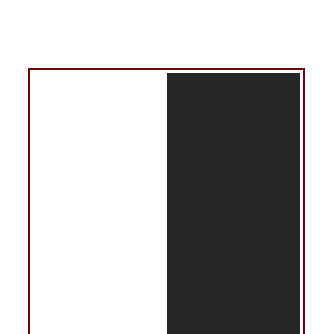
\begin{tikzpicture}
  \draw[thick, USC_Garnet] (0,0) rectangle (3.5,3.5);
  \fill[white] (0.05,0.05) rectangle (1.75,3.45);
  \fill[black!85] (1.75,0.05) rectangle (3.45,3.45);
\end{tikzpicture}\\[0.2cm]
\textbf{(a)} Half-and-half
\end{minipage}
\hfill
\begin{minipage}{0.35\textwidth}\centering
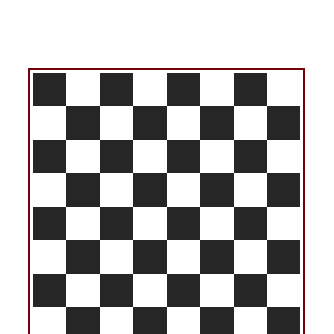
\begin{tikzpicture}
  \draw[thick, USC_Garnet] (0,0) rectangle (3.5,3.5);
  \foreach \i in {0,...,7} {
    \foreach \j in {0,...,7} {
      \pgfmathtruncatemacro{\checkcolor}{mod(\i+\j,2)}
      \ifnum\checkcolor=0
        \fill[white] ({0.05+\i*0.425}, {0.05+\j*0.425}) rectangle ({0.05+\i*0.425+0.425}, {0.05+\j*0.425+0.425});
      \else
        \fill[black!85] ({0.05+\i*0.425}, {0.05+\j*0.425}) rectangle ({0.05+\i*0.425+0.425}, {0.05+\j*0.425+0.425});
      \fi
    }
  }
\end{tikzpicture}\\[0.2cm]
\textbf{(b)} Chessboard
\end{minipage}
\end{center}

\vspace{-0.1cm}

\begin{enumerate}[label=(\alph*)]
\item Would the histogram of the blurred images still be equal? Explain.
\item If your answer is no, sketch the two histograms.
\item \textbf{Bonus question:} Discuss how the histogram of the blurred image (b) is affected by different image size $N$. (5 pts)
\end{enumerate}

\vspace{0.5cm}

\begin{stepbox}[Step 1: Analyze the Original Histograms]
Both images have $N^2/2$ pixels at 0 and $N^2/2$ at 255, so their histograms are identical two-impulse distributions.
\end{stepbox}

\begin{stepbox}[Step 2: Analyze Blurring of Image (a) --- Half-and-Half]
Interior pixels on either side have all 9 neighbors the same color, so they remain at 0 or 255. Only pixels near the vertical split are mixed. For the dominant mixed cases, the $3\times 3$ window has either 3 white + 6 black or 6 white + 3 black pixels, so the blurred values are
\[
\frac{3}{9}\cdot 255 = 85,\qquad \frac{6}{9}\cdot 255 = 170.
\]
So image (a) keeps two strong spikes at 0 and 255, plus much smaller intermediate mass concentrated near 85 and 170 (not centered at 128).
\end{stepbox}

\begin{stepbox}[Step 3: Analyze Blurring of Image (b) --- Chessboard]
For a checkerboard with finite square size, a $3\times 3$ window can contain different counts of white pixels depending on its location relative to square boundaries/corners. If the window contains $k$ white pixels, the output is
\[
r_k=\frac{k}{9}\cdot 255,\qquad k=0,1,\dots,9.
\]
Therefore image (b) has more gray-level variation than image (a), because many different local white/black combinations appear in $3\times 3$ neighborhoods.
\end{stepbox}

\begin{stepbox}[Part (a): Are the Histograms Still Equal?]
\textbf{No.} Image (a) retains most pixels at 0 and 255 with a thin strip of mixed values, mainly near 85 and 170. Image (b) exhibits multiple intermediate levels from different $3\times3$ white/black counts. The histograms differ because the $3\times3$ averaging mask depends on spatial arrangement, not only on the global counts of 0 and 255 pixels.
\end{stepbox}

\begin{stepbox}[Part (b): Sketch of the Two Blurred Histograms]
\begin{center}
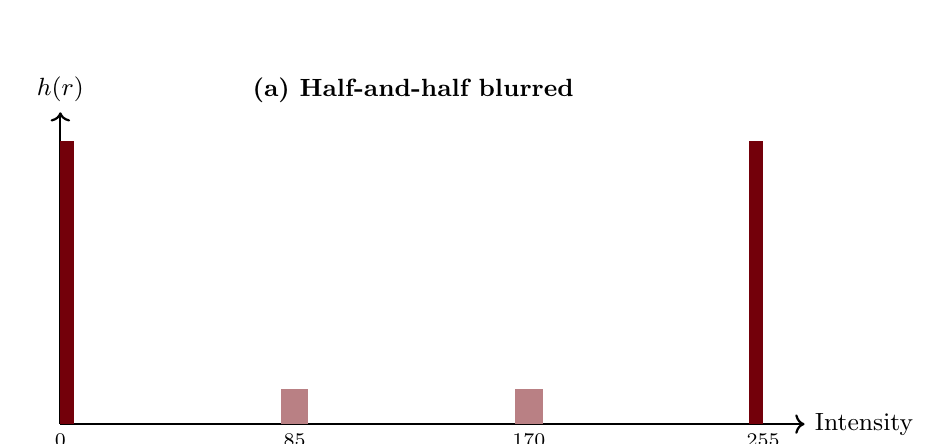
\begin{tikzpicture}[xscale=0.035, yscale=1.8]
% --- Histogram (a): Half-and-half blurred ---
\begin{scope}[shift={(0,0)}]
\draw[->, thick] (0,0) -- (270,0) node[right, font=\small] {Intensity};
\draw[->, thick] (0,0) -- (0,2.2) node[above, font=\small] {$h(r)$};
\node[above, font=\small\bfseries] at (128,2.2) {(a) Half-and-half blurred};
% Large spikes at 0 and 255
\fill[USC_Garnet] (0,0) rectangle (5,2.0);
\fill[USC_Garnet] (250,0) rectangle (255,2.0);
% Small intermediate values near 85 and 170
\fill[USC_Garnet!50] (80,0) rectangle (90,0.25);
\fill[USC_Garnet!50] (165,0) rectangle (175,0.25);
% Tick marks
\node[below, font=\scriptsize] at (0,0) {0};
\node[below, font=\scriptsize] at (85,0) {85};
\node[below, font=\scriptsize] at (170,0) {170};
\node[below, font=\scriptsize] at (255,0) {255};
\end{scope}
\end{tikzpicture}

\vspace{0.5cm}

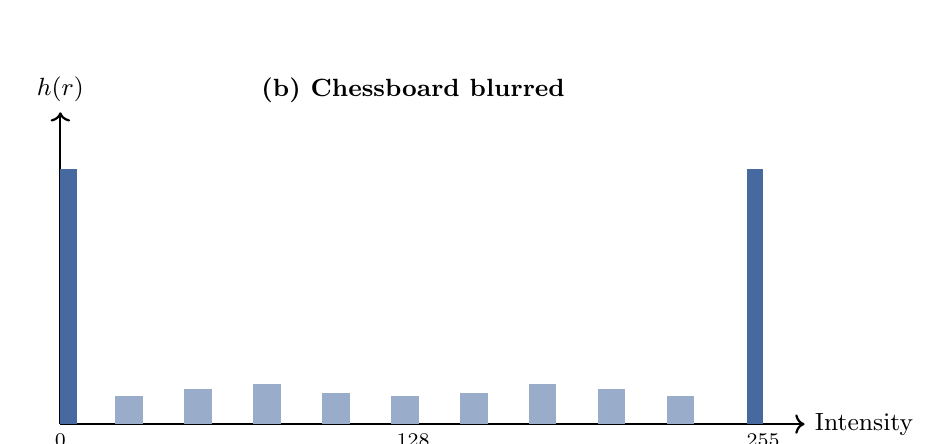
\begin{tikzpicture}[xscale=0.035, yscale=1.8]
% --- Histogram (b): Chessboard blurred ---
\begin{scope}[shift={(0,0)}]
\draw[->, thick] (0,0) -- (270,0) node[right, font=\small] {Intensity};
\draw[->, thick] (0,0) -- (0,2.2) node[above, font=\small] {$h(r)$};
\node[above, font=\small\bfseries] at (128,2.2) {(b) Chessboard blurred};
% Peaks at 0 and 255 with many intermediate levels
\fill[USC_Atlantic] (0,0) rectangle (6,1.8);
\fill[USC_Atlantic] (249,0) rectangle (255,1.8);
\fill[USC_Atlantic!55] (20,0) rectangle (30,0.2);
\fill[USC_Atlantic!55] (45,0) rectangle (55,0.25);
\fill[USC_Atlantic!55] (70,0) rectangle (80,0.28);
\fill[USC_Atlantic!55] (95,0) rectangle (105,0.22);
\fill[USC_Atlantic!55] (120,0) rectangle (130,0.2);
\fill[USC_Atlantic!55] (145,0) rectangle (155,0.22);
\fill[USC_Atlantic!55] (170,0) rectangle (180,0.28);
\fill[USC_Atlantic!55] (195,0) rectangle (205,0.25);
\fill[USC_Atlantic!55] (220,0) rectangle (230,0.2);
% Tick marks
\node[below, font=\scriptsize] at (0,0) {0};
\node[below, font=\scriptsize] at (128,0) {128};
\node[below, font=\scriptsize] at (255,0) {255};
\end{scope}
\end{tikzpicture}
\end{center}
\end{stepbox}

\begin{stepbox}[Part (c) Bonus: Effect of Image Size $N$ on Chessboard Histogram]
As $N$ increases, the fraction of pixels near square boundaries becomes small compared to the total number of interior pixels. Interior pixels remain near pure black or pure white after averaging, while only boundary pixels produce intermediate values. Since the boundary-pixel fraction tends to zero as $N\to\infty$, the histogram approaches two dominant peaks at 0 and 255. For smaller $N$, boundary effects are proportionally larger, so intermediate levels are more visible.
\end{stepbox}

\begin{resultsbox}
\textbf{(a)} No, the histograms of the blurred images are not equal. Image (a) keeps large spikes at 0 and 255, with mixed values mainly near 85 and 170. Image (b) has broader intermediate-level variation because different $3\times3$ neighborhoods contain different white/black counts.

\textbf{(b)} See histogram sketches above. Image (a) is strongly concentrated at the extremes with two minor intermediate components. Image (b) has strong extremes plus a richer spread of intermediate values.

\textbf{(c) Bonus:} As $N \to \infty$, the boundary-affected fraction $\to 0$, so the blurred chessboard histogram is dominated by peaks at 0 and 255. For smaller $N$, boundary mixing contributes more intermediate gray levels.
\end{resultsbox}


% ============================================================================
% PROBLEM 2: Spatial Filtering
% ============================================================================

\question{Problem 2: Spatial Filtering (20 pts)}\label{quest:2}

Consider spatial filtering.

\begin{enumerate}[label=(\alph*)]
\item Suppose that you filter an image $f(x,y)$, with a spatial filter mask $w(x,y)$, using convolution, as defined in Eq.~(3.4-2), where the mask is smaller than the image in both spatial directions. Show the important property that, if the coefficients of the mask sum to zero, then the sum of all the elements in the resulting convolution array (filtered image) will be zero also (you may ignore computational inaccuracies). Also, you may assume that the border of the image has been padded with the appropriate number of zeros. (10 pts)
\begin{align}
w(x,y) \otimes f(x,y) = \sum_{s=-a}^{a} \sum_{t=-b}^{b} w(s,t)\, f(x-s, y-t) \tag{3.4-2}
\end{align}

\item Would the result to (a) be the same if the filtering is implemented using correlation, as defined in Eq.~(3.4-1)? (10 pts)
\begin{align}
w(x,y) \odot f(x,y) = \sum_{s=-a}^{a} \sum_{t=-b}^{b} w(s,t)\, f(x+s, y+t) \tag{3.4-1}
\end{align}
\end{enumerate}

\vspace{0.5cm}

\begin{stepbox}[Part (a): Convolution with Zero-Sum Mask]
Let $g(x,y) = w(x,y) \otimes f(x,y)$ denote the filtered image. We want to show that if $\displaystyle\sum_{s=-a}^{a}\sum_{t=-b}^{b} w(s,t) = 0$, then $\displaystyle\sum_x \sum_y g(x,y) = 0$.
\end{stepbox}

\begin{stepbox}[Step 1: Write the Sum of All Output Pixels]
\[
\sum_x \sum_y g(x,y) = \sum_x \sum_y \sum_{s=-a}^{a} \sum_{t=-b}^{b} w(s,t)\, f(x-s, y-t)
\]
\end{stepbox}

\begin{stepbox}[Step 2: Exchange the Order of Summation]
Since all sums are finite, we can exchange the order:
\[
\sum_x \sum_y g(x,y) = \sum_{s=-a}^{a} \sum_{t=-b}^{b} w(s,t) \left[\sum_x \sum_y f(x-s, y-t)\right]
\]
\end{stepbox}

\begin{stepbox}[Step 3: Evaluate the Inner Sum]
Consider the inner sum $\displaystyle\sum_x \sum_y f(x-s, y-t)$. Substituting $u = x - s$, $v = y - t$ (a change of summation index), and noting that $f$ is zero-padded (i.e., $f(u,v) = 0$ outside the image), the summation range covers all positions where $f$ is nonzero regardless of the shift $(s,t)$. Therefore:
\[
\sum_x \sum_y f(x-s, y-t) = \sum_u \sum_v f(u,v) = S_f \quad \text{(constant, independent of $s,t$)}
\]
where $S_f$ is the sum of all pixel values in the original image.
\end{stepbox}

\begin{stepbox}[Step 4: Factor and Conclude]
Substituting back:
\[
\sum_x \sum_y g(x,y) = \sum_{s=-a}^{a} \sum_{t=-b}^{b} w(s,t) \cdot S_f = S_f \cdot \underbrace{\sum_{s=-a}^{a} \sum_{t=-b}^{b} w(s,t)}_{= \; 0 \text{ (given)}} = 0 \qquad \blacksquare
\]
\end{stepbox}

\begin{stepbox}[Part (b): Correlation with Zero-Sum Mask]
For correlation, $g'(x,y) = \displaystyle\sum_{s=-a}^{a}\sum_{t=-b}^{b} w(s,t)\, f(x+s, y+t)$. The same argument applies:
\[
\sum_x \sum_y g'(x,y) = \sum_{s=-a}^{a}\sum_{t=-b}^{b} w(s,t) \left[\sum_x \sum_y f(x+s, y+t)\right]
\]
With the substitution $u = x+s$, $v = y+t$, the inner sum is again $S_f$ (independent of $s,t$):
\[
\sum_x \sum_y g'(x,y) = S_f \cdot \sum_{s,t} w(s,t) = S_f \cdot 0 = 0 \qquad \blacksquare
\]
\textbf{Yes}, the result is the same for correlation. The sign change in the index ($x-s$ vs.\ $x+s$) does not affect the argument because the inner sum over a shifted version of $f$ always equals $S_f$ under zero-padding.
\end{stepbox}

\begin{resultsbox}
\textbf{(a)} If the mask coefficients sum to zero, i.e., $\sum_{s,t} w(s,t) = 0$, then the sum of all elements in the convolution output is:
\[
\sum_{x,y} g(x,y) = S_f \cdot \sum_{s,t} w(s,t) = 0 \qquad \blacksquare
\]

\textbf{(b)} Yes, the result is identical for correlation. The proof is the same because the inner summation $\sum_{x,y} f(x+s, y+t) = S_f$ is independent of the shift direction. $\blacksquare$
\end{resultsbox}


% ============================================================================
% PROBLEM 3: Averaging Mask and Bar Merging
% ============================================================================

\question{Problem 3: Averaging Mask and Bar Merging (20 pts)}\label{quest:3}

The three images shown were blurred using square averaging masks of sizes $n=23$, 25, and 45, respectively. The vertical bars on the left lower part of (a) and (c) are blurred, but a clear separation exists between them. However, the bars have merged in image (b), in spite of the fact that the mask that produced this image is significantly smaller than the mask that produced image (c).

\vspace{0.5cm}

\begin{center}
\begin{minipage}{0.21\textwidth}\centering
{\color{USC_Garnet}\fbox{\color{black}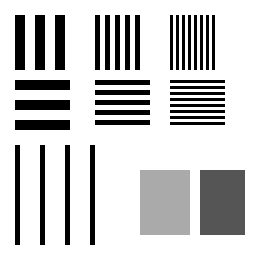
\includegraphics[width=\textwidth]{figures/fig2_original.png}}}\\[0.2cm]
\textbf{Original}
\end{minipage}
\hfill
\begin{minipage}{0.21\textwidth}\centering
{\color{USC_Garnet}\fbox{\color{black}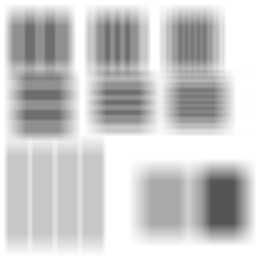
\includegraphics[width=\textwidth]{figures/fig3_a_n23.png}}}\\[0.2cm]
\textbf{(a)} $n=23$
\end{minipage}
\hfill
\begin{minipage}{0.21\textwidth}\centering
{\color{USC_Garnet}\fbox{\color{black}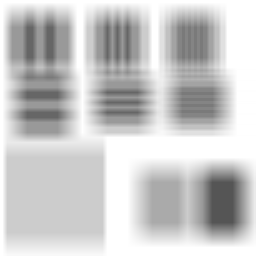
\includegraphics[width=\textwidth]{figures/fig3_b_n25.png}}}\\[0.2cm]
\textbf{(b)} $n=25$
\end{minipage}
\hfill
\begin{minipage}{0.21\textwidth}\centering
{\color{USC_Garnet}\fbox{\color{black}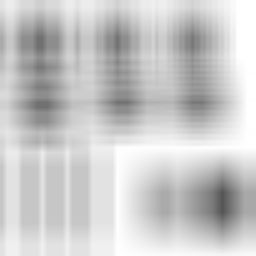
\includegraphics[width=\textwidth]{figures/fig3_c_n45.png}}}\\[0.2cm]
\textbf{(c)} $n=45$
\end{minipage}
\end{center}

\vspace{0.3cm}

Explain the reason for this. The vertical bars are 5 pixels wide, 100 pixels high, and their separation is 20 pixels. (Hints: you can simplify the problem by considering a single scan line through the bars in the image.)

\vspace{0.5cm}

\begin{stepbox}[Step 1: Simplify to a 1D Problem]
Following the hint, consider a single horizontal scan line through the bars. The 1D intensity profile is periodic with bar width 5 pixels (intensity 255), gap width 20 pixels (intensity 0), and \textbf{period $T = 5 + 20 = 25$ pixels}. The $n \times n$ averaging mask reduces to a 1D moving average of width $n$.
\end{stepbox}

\begin{stepbox}[Step 2: Effect of a Moving Average on a Periodic Signal]
A 1D moving average of width $n$ computes:
\[
g(x) = \frac{1}{n}\sum_{k=0}^{n-1} f(x-k)
\]
This sums $n$ consecutive pixels. For a periodic signal with period $T$, the key observation is: if $n$ is an exact multiple of $T$, then the window always contains the same number of ``on'' (bar) and ``off'' (gap) pixels regardless of position, making the output \textbf{constant}.
\end{stepbox}

\begin{stepbox}[Step 3: Why $n = 25$ Causes Complete Merging]
Since $T = 25$ and $n = 25 = 1 \times T$, the averaging window spans \textbf{exactly one full period}. At every position, the window contains exactly 5 bar pixels (at 255) and 20 gap pixels (at 0):
\[
g(x) = \frac{5 \times 255 + 20 \times 0}{25} = \frac{1275}{25} = 51 \quad \text{(constant)}
\]
The output is a uniform gray value of 51 along the entire scan line. All spatial variation is destroyed, and the bars \textbf{merge completely}.
\end{stepbox}

\begin{stepbox}[Visualization: 1D Scan Line Analysis]
\begin{center}
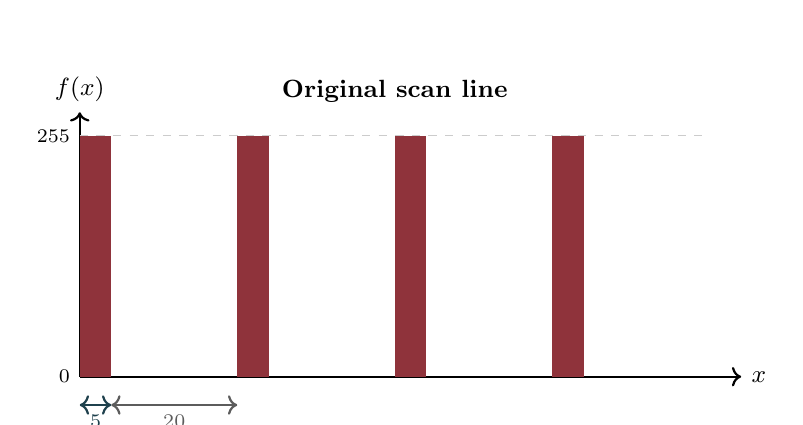
\begin{tikzpicture}[xscale=0.08, yscale=0.012]
% --- Original signal ---
\draw[->, thick] (0,0) -- (105,0) node[right, font=\small] {$x$};
\draw[->, thick] (0,0) -- (0,280) node[above, font=\small] {$f(x)$};
\node[left, font=\scriptsize] at (0,255) {255};
\node[left, font=\scriptsize] at (0,0) {0};
\draw[dashed, gray!40] (0,255) -- (100,255);
% Draw bars (4 bars, period 25)
\foreach \i in {0,...,3} {
  \fill[USC_Garnet!80] ({\i*25},0) rectangle ({\i*25+5},255);
}
\node[above, font=\small\bfseries] at (50,280) {Original scan line};
% Dimension annotations
\draw[<->, thick, USC_Congaree] (0,-30) -- (5,-30);
\node[below, font=\scriptsize, USC_Congaree] at (2.5,-30) {5};
\draw[<->, thick, USC_Black70] (5,-30) -- (25,-30);
\node[below, font=\scriptsize, USC_Black70] at (15,-30) {20};
\end{tikzpicture}

\vspace{0.3cm}

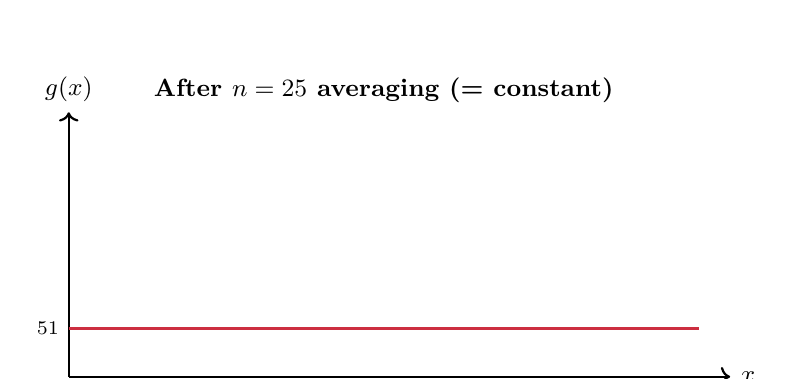
\begin{tikzpicture}[xscale=0.08, yscale=0.012]
% --- n=25 output ---
\draw[->, thick] (0,0) -- (105,0) node[right, font=\small] {$x$};
\draw[->, thick] (0,0) -- (0,280) node[above, font=\small] {$g(x)$};
\node[left, font=\scriptsize] at (0,51) {51};
\draw[thick, USC_Rose] (0,51) -- (100,51);
\node[above, font=\small\bfseries] at (50,280) {After $n=25$ averaging (= constant)};
\end{tikzpicture}
\end{center}
\end{stepbox}

\begin{stepbox}[Step 4: Why $n = 23$ and $n = 45$ Preserve Separation]
\textbf{$n = 23 < T$:} The window is smaller than one period, so the number of bar pixels it covers varies with position, preserving the intensity modulation.

\textbf{$n = 45 \neq kT$:} Since $45 = 25 + 20$ is not a multiple of $T$, the window alternates between covering 1 and 2 bars. The output is more blurred but spatial variation persists.
\end{stepbox}

\begin{resultsbox}
The bars merge completely when $n = 25$ because the averaging mask width \textbf{exactly matches the period} of the bar pattern ($T = 5 + 20 = 25$ pixels). When $n = T$, the moving average window always contains the same number of bar and gap pixels at every position, producing a constant output and destroying all spatial variation.

For $n = 23 < T$ and $n = 45 \neq kT$, the window size does not match the period, so the number of bar pixels in the window varies with position, preserving the intensity modulation and keeping the bars distinguishable. $\blacksquare$
\end{resultsbox}


% ============================================================================
% PROBLEM 4: Averaging and Laplacian Order
% ============================================================================

\question{Problem 4: Averaging and Laplacian Order (20 pts)}\label{quest:4}

In a given application an averaging mask is applied to input images to reduce noise, and then a Laplacian mask is applied to enhance small details. Would the result be the same if the order of these operations were reversed?

\vspace{0.5cm}

\begin{stepbox}[Step 1: Express Both Operations as Convolutions]
Let $w_{\text{avg}}$ denote the averaging mask and $w_{\text{lap}}$ denote the Laplacian mask. Both are linear spatial filters, so both operations are convolutions:
\[
g_1 = w_{\text{lap}} \otimes (w_{\text{avg}} \otimes f) \qquad \text{(average first, then Laplacian)}
\]
\[
g_2 = w_{\text{avg}} \otimes (w_{\text{lap}} \otimes f) \qquad \text{(Laplacian first, then average)}
\]
\end{stepbox}

\begin{stepbox}[Step 2: Apply Associativity and Commutativity of Convolution]
Convolution is both \textbf{associative} and \textbf{commutative}:
\[
w_1 \otimes (w_2 \otimes f) = (w_1 \otimes w_2) \otimes f = (w_2 \otimes w_1) \otimes f = w_2 \otimes (w_1 \otimes f)
\]
Applying this to our operations:
\[
g_1 = w_{\text{lap}} \otimes (w_{\text{avg}} \otimes f) = (w_{\text{lap}} \otimes w_{\text{avg}}) \otimes f
\]
\[
g_2 = w_{\text{avg}} \otimes (w_{\text{lap}} \otimes f) = (w_{\text{avg}} \otimes w_{\text{lap}}) \otimes f
\]
Since $w_{\text{lap}} \otimes w_{\text{avg}} = w_{\text{avg}} \otimes w_{\text{lap}}$ (commutativity), we have:
\[
g_1 = g_2
\]
\end{stepbox}

\begin{resultsbox}
\textbf{Yes}, the result is the same regardless of the order. Both the averaging mask and the Laplacian mask are linear, shift-invariant operators (i.e., convolutions). Since convolution is associative and commutative:
\[
w_{\text{lap}} \otimes (w_{\text{avg}} \otimes f) = w_{\text{avg}} \otimes (w_{\text{lap}} \otimes f)
\]
The mathematical output is identical. $\blacksquare$
\end{resultsbox}


% ============================================================================
% PROBLEM 5: Convolution Filtering
% ============================================================================

\question{Problem 5: Convolution Filtering (20 pts)}\label{quest:5}

Given the following $3 \times 3$ filter, perform the image filtering using \textbf{convolution}. Give the \textbf{FULL} filtering result for each filtering process. (Hint: you need to assume an appropriate zero mapping.)
%
\[
w = \begin{bmatrix} -1 & 0 & -1 \\ 0 & 2 & 0 \\ 1 & 0 & 1 \end{bmatrix}
\]
%
\begin{enumerate}[label=(\alph*)]
\item a $2 \times 2$ image as shown in image (a) \hfill (10 pts)
\item a $3 \times 3$ image as shown in image (b) \hfill (10 pts)
\end{enumerate}

\vspace{0.5cm}

\begin{center}
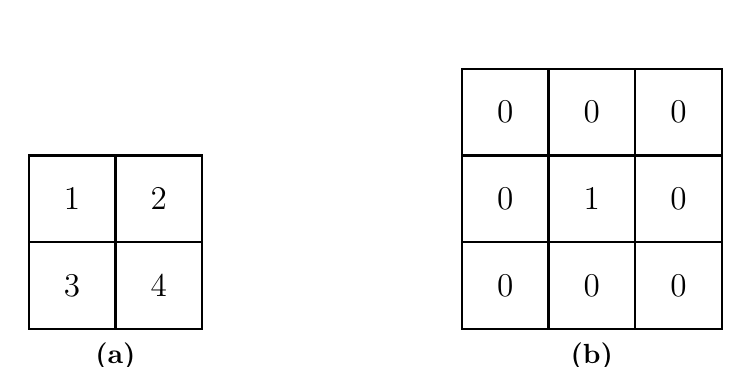
\begin{tikzpicture}[
  imgcell/.style={minimum size=1.1cm, draw=black, thick, fill=white, font=\large\bfseries},
  gridcell/.style={minimum size=1.1cm, draw=black, thick, fill=white, font=\large\bfseries},
]

% --- (a) 2x2 image ---
\node[imgcell] at (0, 1.1) {$1$};
\node[imgcell] at (1.1, 1.1) {$2$};
\node[imgcell] at (0, 0) {$3$};
\node[imgcell] at (1.1, 0) {$4$};
\node[font=\bfseries] at (0.55, -0.9) {(a)};

% --- (b) 3x3 identity image ---
\foreach \val/\col/\row in {
  0/0/2, 0/1/2, 0/2/2,
  0/0/1, 1/1/1, 0/2/1,
  0/0/0, 0/1/0, 0/2/0}
{
  \node[gridcell] at (5.5+\col*1.1, \row*1.1) {$\val$};
}
\node[font=\bfseries] at (6.6, -0.9) {(b)};

\end{tikzpicture}
\end{center}

\vspace{0.5cm}

\begin{stepbox}[Setup: Convolution Formula]
The convolution is defined as:
\[
g(x,y) = \sum_{s=-1}^{1}\sum_{t=-1}^{1} w(s,t)\, f(x-s, y-t)
\]
where $f(x,y) = 0$ outside the image (zero-padding). Because the problem asks for \textbf{FULL} convolution, the output size is $(M+2)\times(N+2)$ for an $M\times N$ input and a $3\times3$ mask.

The mask $w$ with indices $s,t \in \{-1, 0, 1\}$:
\[
w(-1,-1) = -1,\; w(-1,0) = 0,\; w(-1,1) = -1
\]
\[
w(0,-1) = 0,\; w(0,0) = 2,\; w(0,1) = 0
\]
\[
w(1,-1) = 1,\; w(1,0) = 0,\; w(1,1) = 1
\]
\end{stepbox}

\begin{stepbox}[Part (a): $2 \times 2$ Image $\to$ $4 \times 4$ FULL Output]
Image: $f(0,0) = 1$, $f(0,1) = 2$, $f(1,0) = 3$, $f(1,1) = 4$. All other $f = 0$ (zero-padded border).

The full convolution result is:
\[
g_{\text{full}}=
\begin{bmatrix}
-1 & -2 & -1 & -2 \\
-3 & -2 & 1 & -4 \\
1 & 8 & 9 & 2 \\
3 & 4 & 3 & 4
\end{bmatrix}.
\]
\end{stepbox}

\begin{stepbox}[Part (a) Result Grid]
\begin{center}
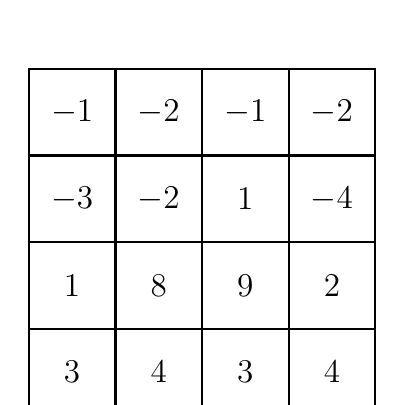
\begin{tikzpicture}[
  cell/.style={minimum size=1.1cm, draw=black, thick, fill=white, font=\large\bfseries},
]
\node[cell] at (0,3.3) {$-1$};
\node[cell] at (1.1,3.3) {$-2$};
\node[cell] at (2.2,3.3) {$-1$};
\node[cell] at (3.3,3.3) {$-2$};

\node[cell] at (0,2.2) {$-3$};
\node[cell] at (1.1,2.2) {$-2$};
\node[cell] at (2.2,2.2) {$1$};
\node[cell] at (3.3,2.2) {$-4$};

\node[cell] at (0,1.1) {$1$};
\node[cell] at (1.1,1.1) {$8$};
\node[cell] at (2.2,1.1) {$9$};
\node[cell] at (3.3,1.1) {$2$};

\node[cell] at (0,0) {$3$};
\node[cell] at (1.1,0) {$4$};
\node[cell] at (2.2,0) {$3$};
\node[cell] at (3.3,0) {$4$};
\end{tikzpicture}
\end{center}
\end{stepbox}

\begin{stepbox}[Part (b): $3 \times 3$ Image $\to$ $5 \times 5$ FULL Output]
Image: $f(1,1) = 1$, all other $f(i,j) = 0$. This is a unit impulse at position $(1,1)$.

For full convolution, the impulse response appears centered in the $5\times5$ output support:
\[
g_{\text{full}}=
\begin{bmatrix}
0 & 0 & 0 & 0 & 0 \\
0 & -1 & 0 & -1 & 0 \\
0 & 0 & 2 & 0 & 0 \\
0 & 1 & 0 & 1 & 0 \\
0 & 0 & 0 & 0 & 0
\end{bmatrix}.
\]
\end{stepbox}

\begin{stepbox}[Part (b) Result Grid]
\begin{center}
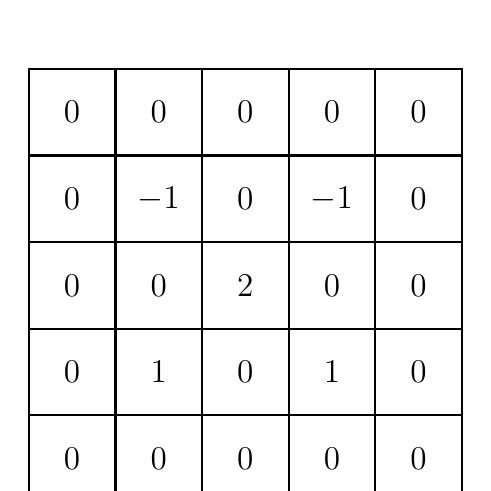
\begin{tikzpicture}[
  cell/.style={minimum size=1.1cm, draw=black, thick, fill=white, font=\large\bfseries},
]
\node[cell] at (0,4.4) {$0$};
\node[cell] at (1.1,4.4) {$0$};
\node[cell] at (2.2,4.4) {$0$};
\node[cell] at (3.3,4.4) {$0$};
\node[cell] at (4.4,4.4) {$0$};

\node[cell] at (0,3.3) {$0$};
\node[cell] at (1.1,3.3) {$-1$};
\node[cell] at (2.2,3.3) {$0$};
\node[cell] at (3.3,3.3) {$-1$};
\node[cell] at (4.4,3.3) {$0$};

\node[cell] at (0,2.2) {$0$};
\node[cell] at (1.1,2.2) {$0$};
\node[cell] at (2.2,2.2) {$2$};
\node[cell] at (3.3,2.2) {$0$};
\node[cell] at (4.4,2.2) {$0$};

\node[cell] at (0,1.1) {$0$};
\node[cell] at (1.1,1.1) {$1$};
\node[cell] at (2.2,1.1) {$0$};
\node[cell] at (3.3,1.1) {$1$};
\node[cell] at (4.4,1.1) {$0$};

\node[cell] at (0,0) {$0$};
\node[cell] at (1.1,0) {$0$};
\node[cell] at (2.2,0) {$0$};
\node[cell] at (3.3,0) {$0$};
\node[cell] at (4.4,0) {$0$};
\end{tikzpicture}
\end{center}

The central $3\times3$ block equals the filter response around the impulse location, embedded in the full $5\times5$ support. $\blacksquare$
\end{stepbox}

\begin{resultsbox}
\textbf{(a)} The full convolution output ($2\times2$ image with $3\times3$ mask) is:
\[
g_{\text{full}}=
\begin{bmatrix}
-1 & -2 & -1 & -2 \\
-3 & -2 & 1 & -4 \\
1 & 8 & 9 & 2 \\
3 & 4 & 3 & 4
\end{bmatrix}
\]

\textbf{(b)} The full convolution output ($3\times3$ impulse image with $3\times3$ mask) is:
\[
g_{\text{full}}=
\begin{bmatrix}
0 & 0 & 0 & 0 & 0 \\
0 & -1 & 0 & -1 & 0 \\
0 & 0 & 2 & 0 & 0 \\
0 & 1 & 0 & 1 & 0 \\
0 & 0 & 0 & 0 & 0
\end{bmatrix}
\qquad \blacksquare
\]
\end{resultsbox}


% ============================================================================
% END OF DOCUMENT
% ============================================================================

\end{document}
